
\chapter[Introdução]{Introdução}
%\addcontentsline{toc}{chapter}{Introdução}
% ----------------------------------------------------------

\section{Motivação}

O problema de buscar o melhor caminho entre dois pontos tem uma grande importância em areas como da engenharia e ciência, tais como rotear o trafico de telefone, navegar por um labirinto ou mesmo definir o layout de trilhas impressas em uma placa eletrônica.

Busca de caminhos também tem uma grande importância no âmbito dos jogos digitais, onde um jogador compete ou coopera com uma inteligencia artificial e é preciso chegar ao seu destino de forma competente, como por exemplo, jogos de tiro em primeira pessoa ou de estrategia em tempo real.

O valor de entretenimento do jogo pode ser drasticamente reduzido, quando os personagens não podem atravessar um mapa complexo de forma competente, podendo afetar a experiencia de jogo ao deixar visível para o jogador a sua incapacidade de lidar com a busca de caminho de forma satisfatória.

Ainda é comum, em jogos digitais, termos mais de um agente de busca de caminho ao mesmo tempo no mesmo cenário, podendo ser muitas vezes muito custoso computacionalmente falando. Por isso vários desenvolvedores de jogos têm juntado esforços para desenvolver soluções de busca de caminho em ambientes de recursos escassos.



\cite{Pontevia}

%\section{Justificativa}

Muitas abordagens para melhorar o desempenho ou diminuir o custo de métodos de busca de caminho tem sido desenvolvidos \cite{Ulysses}  \cite{Pollack} \cite{Timothy} \cite{WilliamMiller}. 

Ainda temos problemas de alto custo computacional, que para serem minimizados em alguns casos, acabamos sacrificando a certeza de melhor caminho por um melhor desempenho\cite{Botea}\cite{KORF199341}. Por isso iremos fazer uma análise e propor um modelo para otimizar alguma limitação do modelo, visando em principal o âmbito dos jogos digitais.

Qualquer problema que possa ser formulado em busca em grafos pode solucionado a partir de busca heuristicas. O exemplo mais comum problema que podem ser resuzido é o PCV, outro exemplo tipico é quebra cabeça de delizar, que consiste em quadro que contem quadrados numerados e uma posição vazia (ver \ref{fig:GrafoBusca}). As operações permitidas são deslizar qualquer peça horizontalmente ou verticalmente adjacente a peça vazia para a posição vazia, o objetivo é rearranjar as peças a partir de uma confiruação randomica com menor quantidade de movimentos. Encontrar a solução otima para esse problema ou para o PCF é NP-Completo. \cite{Kar72} \cite{RatnerW86}

\begin{minipage}{\linewidth}
    \makebox[\linewidth]{
        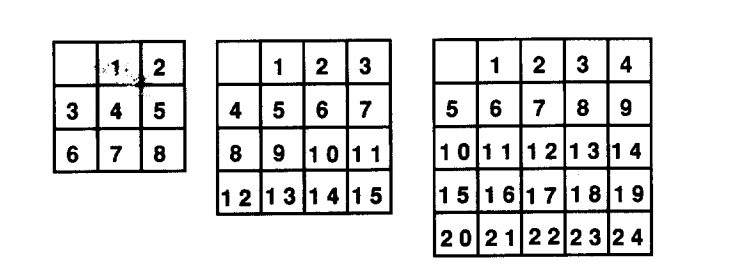
\includegraphics[keepaspectratio=true,scale=0.8]{ibagens/slide-puzzle.png}}
    \captionof{figure}{Quebra cabeça de deslizar \cite{KORF199341}}
    \label{fig:slide-puzzle}
\end{minipage}

Este cenário é a principal motivação deste trabalho que consiste em propor, implementar e mensurar resultados de uma solução para busca de melhor caminho entre dois pontos.

\section{Objetivos}

Este trabalho tem como objetivo verificar a aplicabilidade de paralelismo de AG para melhoria de precisão em busca heurística de caminhos. O ponto central é a definição de uma estrutura capaz de explorar as vantagens demonstradas no uso de AG com computação paralela e aplica-las em um modelo de busca heurística de caminho que use AG para redução de custo de memória e processamento, ja que para isto, estes tendem a sacrificar a certeza de encontrar a menor rota. 

Implementar o modelo de busca heurística com AG e mensurar os resultados. 

Aplicar um modelo de paralelização de AG. 

Combinar o modelo paralelo com o de busca e mensurar os resultados.


\section{Método de trabalho}

Primeiramente sera desenvolvido uma bateria de testes de caminhos, com intuito de terem diferentes tamanhos, levando em cosideração mapas com padrões de repetição e sem padrões de repetição, os mesmos serão modelados de forma bidimensional em arquivos de texto com caracteres para definir o ponto inicial (S), final (E), obstáculos (\#) e caminho livre (.).

Será implementada a busca heuristica A* utilizando a linguagem C\# .NET, levando em consideração os arquivos de teste desenvolvidos como entrada, retornando se existe um caminho entre o ponto inicial e final, quanto tempo levou para encontrar o caminho e consumo de memoria para chegar na solução. 

Também será implementado um AG para utilizar em conjunto ao A*, também utilizando a linguagem C\# .NET, implementando o mesmo método proposto por Ulysses O. Santos \cite{Ulysses}. A implementação receberá  arquivos de testes de entrada contendo os mapas, os mesmos  utilizado para testar a implementação do A* anteriormente, tambem retornando o tempo e consumo de memoria para chegar na solução.
Os parâmetros utilizados para o AG serão uma população inicial de 4 indivíduos, com o critério de geração de descendentes em 50\%, com o critério de mutação em 25\% e será calculada a aptidão para 12 indivíduos.

Por ultimo, será implementado uma modificação do AG para paraleliza-lo, como proposto por \cite{Alaoui}. Serão utilizadas N \textit{threads} para a separação das populações, ou seja, trabalhando com varias populações ao mesmo tempo, onde cada \textit{thread} fica responsavel por uma, para depois mesclar os melhores individuos entre elas, esse sistema ira receber os mesmo arquivos de testes utilizados nas implementações anteriores, retornando informações de tempo e consumo de memória.

Nas três implementações todos os testes serão executados 100 vezes e será calcula a média do tempo e consumo de memoria de cada um. Todos os dados coletados serão comparados em forma de tabelas e gráficos, para demostrar os ganhos e perdas relativos de cada abordagem.




\section{Organização do trabalho}


